\documentclass[12pt, titlepage]{article}

\usepackage{amsmath, mathtools}
\usepackage{amsfonts}
\usepackage{amssymb}
\usepackage{colortbl}
\usepackage{xr}
\usepackage{hyperref}
\usepackage{longtable}
\usepackage{xfrac}
\usepackage{tabularx}
\usepackage{siunitx}
\usepackage{caption}
\usepackage{pdflscape}
\usepackage{afterpage}
\usepackage{verbatim}
\usepackage[round]{natbib}
\usepackage{colortbl}
\usepackage{hyperref}
\usepackage{lingmacros}
\usepackage{tree-dvips}
\usepackage{blindtext}
\usepackage{colortbl}%For FR tables
\usepackage{hyperref}%For advanced hyperlinks
\usepackage{enumitem}%For advanced lists
\usepackage{pdfpages}
\usepackage{array}
\usepackage{tikz}

\usepackage{fullpage}
\usepackage{multirow}
\usepackage{booktabs}
\usepackage{graphicx}
\usepackage{float}
\usepackage[toc,page]{appendix}
\hypersetup{
    colorlinks,
    citecolor=blue,
    filecolor=black,
    linkcolor=red,
    urlcolor=blue
}

%% Comments

\usepackage{color}

\newif\ifcomments\commentstrue %displays comments
%\newif\ifcomments\commentsfalse %so that comments do not display

\ifcomments
\newcommand{\authornote}[3]{\textcolor{#1}{[#3 ---#2]}}
\newcommand{\todo}[1]{\textcolor{red}{[TODO: #1]}}
\else
\newcommand{\authornote}[3]{}
\newcommand{\todo}[1]{}
\fi

\newcommand{\wss}[1]{\authornote{blue}{SS}{#1}} 
\newcommand{\plt}[1]{\authornote{magenta}{TPLT}{#1}} %For explanation of the template
\newcommand{\an}[1]{\authornote{cyan}{Author}{#1}}

%% Common Parts

\newcommand{\progname}{ProgName} % PUT YOUR PROGRAM NAME HERE
\newcommand{\authname}{Team \#, Team Name
\\ Student 1 name
\\ Student 2 name
\\ Student 3 name
\\ Student 4 name} % AUTHOR NAMES                  

\usepackage{hyperref}
    \hypersetup{colorlinks=true, linkcolor=blue, citecolor=blue, filecolor=blue,
                urlcolor=blue, unicode=false}
    \urlstyle{same}
                                


\newcounter{acnum}
\newcommand{\actheacnum}{AC\theacnum}
\newcommand{\acref}[1]{AC\ref{#1}}

\newcounter{ucnum}
\newcommand{\uctheucnum}{UC\theucnum}
\newcommand{\uref}[1]{UC\ref{#1}}

\newcounter{mnum}
\newcommand{\mthemnum}{M\themnum}
\newcommand{\mref}[1]{M\ref{#1}}

\begin{document}

\title{System Design for \progname{}} 
\author{\authname}
\date{\today}

\maketitle

\pagenumbering{roman}

\section*{Revision History}

\begin{tabularx}{\textwidth}{p{3cm}p{2cm}X}
\toprule {\bf Date} & {\bf Version} & {\bf Notes}\\
\midrule
Date 1 & 1.0 & Notes\\
Date 2 & 1.1 & Notes\\
\bottomrule
\end{tabularx}

\newpage

\section*{Reference Material}

This section records information for easy reference.

\subsection*{Abbreviations and Acronyms}

\renewcommand{\arraystretch}{1.2}
\begin{tabular}{l l} 
  \toprule		
  \textbf{symbol} & \textbf{description}\\
  \midrule 
  \progname & Explanation of program name\\
  \wss{...} & \wss{...}\\
  \bottomrule
\end{tabular}\\

\newpage

\tableofcontents

\newpage

\listoftables

\listoffigures

\newpage

\pagenumbering{arabic}

\section{Introduction}
Synesthesia Wear is a wearable product that assists users with certain vocal tasks 
that need attention. These tasks can be generic or custom to the user as needed. 
Furthermore, the product will use signal processing to gather and analyze information 
to determine the best and most appropriate feedback (via vibrations) to send to the 
user. As a result, this gives the users peace of mind knowing that if their attention 
is needed (doorbell, ring, name call, etc.), Synesthesia Wear will be able to alert them.

\section{Purpose}
The purpose of this document is to be able to identify and elaborate on all aspects of design involved
in the creation of the Synesthesia Wear system. This involves decomposing the system into different categories and components 
that all have an impact on the system's overall design and functionality.

To add on, this document is intended to be viewed in conjunction with the \href{https://github.com/jordanbierbrier/capstone/blob/main/docs/Design/SoftArchitecture/MG.pdf}{\textit{MG.pdf}} (Software Architecture Design) 
and the \href{https://github.com/jordanbierbrier/capstone/blob/main/docs/Design/SoftDetailedDes/MIS.pdf}{\textit{MIS.pdf}} (Detailed Design) documents so that readers may have a full comprehension on the many aspects of Synesthesia 
Wear's design in its entirety. 

\section{Scope}
\subsection {Document Scope}
As stated before, this document will split up the system design into different categories and components 
such that the readers may be able to better understand each components impact on the system's functionality/completeness.\\\\
\noindent With the above in mind, the scope of this document will involve:
\begin{itemize}
  \item \textbf{Project Overview:} This section goes over the system's behaviour, undesired event handling, system components, and requirement-design connections.  
  \item \textbf{System Variables:} As its name suggests, this section goes over variables/aspects to the system that has the potential to change.
  \item \textbf{User Interfaces:} This section involves elaborating on the interfaces that users interact with when using the Synesthesia Wear system.
  \item \textbf{Design of Mechanical Hardware:} In this section, details on what will be built, fabrication, materials, and drawings/sketches for mechanical components will be discussed in further detail. 
  \item \textbf{Design of Electrical Components:} Similar to design of hardware, this section will instead involve details regarding electrical components.
  \item \textbf{Design of Communication Protocols:} For this section, details on the communication protocols used in the Synesthesia Wear system will be discussed.
  \item \textbf{Timeline:} This section will go over the schedules of all remaining tasks for Rev 0 and which team member will be responsible for each task's completion.
\end{itemize}

\subsection {Assumptions}
The system is designed with the following assumptions:
\begin{table}[H]
  \centering
  \arrayrulecolor{white}
  \begin{tabular}{|p{3cm}|p{11cm}|} 
  \hline
  \rowcolor[rgb]{0.071,0.49,0.698} \textcolor{white}{A1} & \textcolor{white}{Each user has a device and WIFI capable of installing the Synesthesia Wear application.}                                          \\ 
  \hline
  \rowcolor[rgb]{0.675,0.827,0.902} Rationale               & Without a device and/or internet connection, the user will be unable to benefit from using Synesthesia Wear.\\
  \hline
  \end{tabular}
  \arrayrulecolor{black}
\end{table}

\begin{table}[H]
  \centering
  \arrayrulecolor{white}
  \begin{tabular}{|p{3cm}|p{11cm}|} 
  \hline
  \rowcolor[rgb]{0.071,0.49,0.698} \textcolor{white}{A2} & \textcolor{white}{The users set their sound configurations to realistic daily-life sounds.}                                    \\ 
  \hline
  \rowcolor[rgb]{0.675,0.827,0.902} Rationale               & The system would be inaccurate when trying to process \quad imaginary or rare sounds with a lack of audio samples (like a meteor crash).\\
  \hline
  \end{tabular}
  \arrayrulecolor{black}
\end{table}

The following are in reference to the critical assumptions in Synesthesia Wear's

\href{https://github.com/jordanbierbrier/capstone/blob/main/docs/HazardAnalysis/HazardAnalysis.pdf}{\textit{HazardAnalysis.pdf}} document:

\begin{table}[H]
  \centering
  \arrayrulecolor{white}
  \begin{tabular}{|p{3cm}|p{11cm}|} 
  \hline
  \rowcolor[rgb]{0.071,0.49,0.698} \textcolor{white}{A3} & \textcolor{white}{The battery will not need to be replaced during product \quad lifespan.}                                          \\ 
  \hline
  \rowcolor[rgb]{0.675,0.827,0.902} Rationale               & It is undesirable and annoying for users if they had to replace the battery frequently during use.\\
  \hline
  \end{tabular}
  \arrayrulecolor{black}
\end{table}

\begin{table}[H]
  \centering
  \arrayrulecolor{white}
  \begin{tabular}{|p{3cm}|p{11cm}|} 
  \hline
  \rowcolor[rgb]{0.071,0.49,0.698} \textcolor{white}{A4} & \textcolor{white}{The microphone is not blocked and has realistic access to the environment.}                                          \\ 
  \hline
  \rowcolor[rgb]{0.675,0.827,0.902} Rationale               & If the microphone is intentionally blocked or put into an environment that hinders its detection (anechoic chamber), it is unreasonable to expect accurate results.\\
  \hline
  \end{tabular}
  \arrayrulecolor{black}
\end{table}




\subsection {System Context}
\begin{figure}[H]
  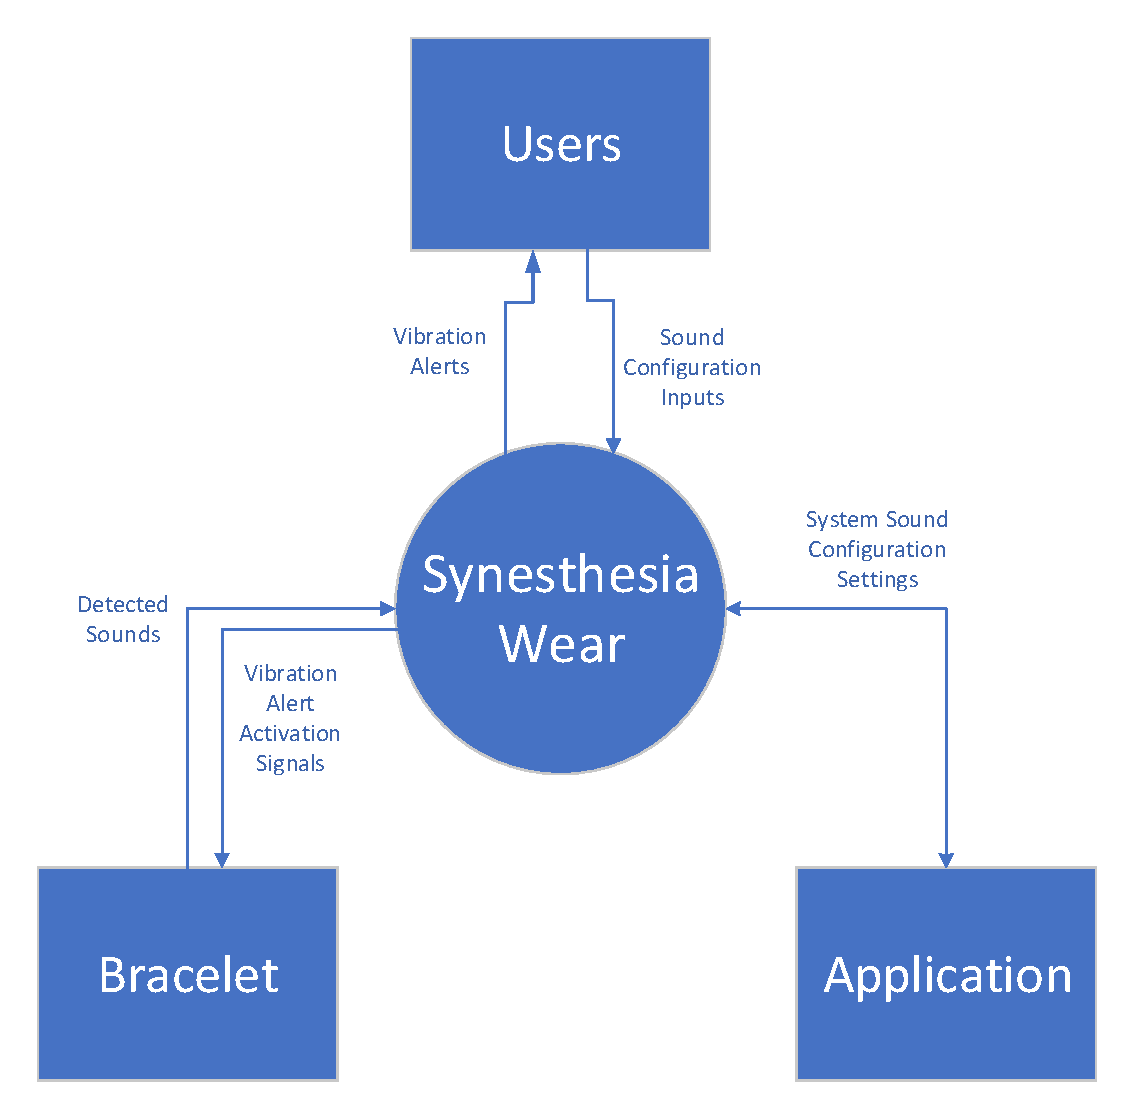
\includegraphics[width=\textwidth,height=\textheight,keepaspectratio]{ContextDiagram.pdf}
  \caption{System Context Diagram}
  \label{ContextDiagram} 
\end{figure}

\newpage

\section{Project Overview}

\subsection{Normal Behaviour}
When starting off, the users should strap the Synesthesia Wear bracelet onto either of their wrists as it was intended.
Afterwards, users would have to install the Synesthesia Wear app onto a device of their choice and possibly look through the app 
to get more familiar with its features and user interface. When ready, the user would then input their desired sound configuration 
settings into the app and then save them so that the app can send these settings over to the bracelet for configurations.
Once recieved, the bracelet can then start to detect for sounds where its built-in microcontroller will process these sounds and try to 
match it with the sounds configured in the settings. Lastly, once a detected sound has ``accurately'' (according to Machine Learning Algorithm) matched a configured sound, a vibration 
alert signal will be sent to the built-in vibration motor which will notify the user that their attention is needed.

\subsection{Undesired Event Handling}
For undesired events, 

\subsection{Component Diagram}

\subsection{Connection Between Requirements and Design} \label{SecConnection}

\wss{The intention of this section is to document decisions that are made
  ``between'' the requirements and the design.  To satisfy some requirements,
  design decisions need to be made.  Rather than make these decisions implicit,
  they are explicitly recorded here.  For instance, if a program has security
  requirements, a specific design decision may be made to satisfy those
  requirements with a password.}

\section{System Variables}

\wss{Include this section for Mechatronics projects}

\subsection{Monitored Variables}

\subsection{Controlled Variables}

\subsection{Constants Variables}

\section{User Interfaces}

\wss{Design of user interface for software and hardware.  Attach an appendix if
needed. Drawings, Sketches, Figma}

\section{Design of Mechanical Hardware}

\wss{Most relevant for mechatronics projects}
\wss{Show what will be acquired}
\wss{Show what will be built, with detail on fabrication and materials}
\wss{Include appendices as appropriate, possibly with sketches, drawings, CAD, etc}

\section{Design of Electrical Components}
\vspace*{-0.5cm}
\begin{table}[H]
  \caption{Electrical Components List}
  \scriptsize	
  \vspace*{-0.5cm}
  \begin{center}
  \begin{tabular}{| p{0.25\textwidth} | p{0.08\textwidth}  | p{0.10\textwidth} | p{0.15\textwidth} | p{0.30\textwidth} |}
   \hline
  \textbf{Component} & \textbf{Amount} & \textbf{Cost \quad \quad (in CAD\$)} & \textbf{Dimensions} & \textbf{Link} \\ \hline

  Arduino Nano 33 BLE	& 2 & 80 & 48 * 18 & 	\url{https://www.amazon.ca/Arduino-Nano-33-BLE-Sense/dp/B07WV5GF17} \\ \hline
  Lithium-Ion Polymer (LiPo) Battery (3.7V 1000mAh)	& 1	& 10 & 50*32*5 & 	\url{https://www.canadarobotix.com/products/588} \\ \hline
  0.1 microfarad capacitor	& 2 &	1.11 &	5*3	& \url{https://rb.gy/vyewya} \\ \hline
  Resistor 1000 ohm	& 1	& NA &	5*3 &	At home \\ \hline
  Resistor 20 ohm &	1 &	NA &	5*3 &	At home \\ \hline
  Vibration motor &	5 &	10 &	10*2 &	\url{https://www.amazon.ca/dp/B089NTLLWB?ref_=cm_sw_r_apin_dp_YEQ7CS0SNQV7HKHZZVFD} \\ \hline
  Transistor NPN - PN2222 &	1 &	NA &	5*3 &	At home \\ \hline
  Diode - IN4007 &	1 & 	NA &	5*3 &	At home \\ \hline
  Power Management module & 2 &	17.5 &	35*22 &	\url{https://www.digikey.com/en/products/detail/sparkfun-electronics/PRT-14411/1568-1723-ND/7725301} \\ \hline

  \end{tabular}
  \end{center}
  \hspace*{-1cm}
  \end{table}

\wss{Most relevant for mechatronics projects}
\wss{Show what will be acquired}
\wss{Show what will be built, with detail on fabrication and materials}
\wss{Include appendices as appropriate, possibly with sketches, drawings,
circuit diagrams, etc}

\section{Design of Communication Protocols}

\wss{If appropriate}

\section{Timeline}

\wss{Schedule of tasks and who is responsible}

% \bibliographystyle {plainnat}
% \bibliography{../../../refs/References}

\newpage{}

\begin{appendices}
  \section{Interface}
  \label{appendix:interface}
  \wss{Include additional information related to the appearance of, and
  interaction with, the user interface}
  
  \section{Mechanical Hardware}
  \label{appendix:hardware}
  
  \section{Electrical Components}
  \label{appendix:electrical}
  
  \section{Communication Protocols}
  \label{appendix:protocols}
  
  \section{Reflection}
  \label{appendix:reflection}
  
  The information in this section will be used to evaluate the team members on the
  graduate attribute of Problem Analysis and Design.  Please answer the following questions:
  
  \begin{enumerate}
    \item What are the limitations of your solution?  Put another way, given
    unlimited resources, what could you do to make the project better? (LO\_ProbSolutions)
    \item Give a brief overview of other design solutions you considered.  What
    are the benefits and tradeoffs of those other designs compared with the chosen
    design?  From all the potential options, why did you select documented design?
    (LO\_Explores)
  \end{enumerate}
  
  \end{appendices}
\end{document}